\documentclass{beamer}


\usepackage{graphicx}
\usepackage{latexsym}
\usepackage{amsmath}
\usepackage{wrapfig}
\usepackage{algorithmic}
\usepackage[boxed]{algorithm}
\usepackage{rotating}
\usepackage{fancybox}
\usepackage{hyperref}
\usepackage{verbatim}
\usepackage{color}
\usepackage{multicol}
\usepackage{lmodern} % to allow arbitrary font sizes

\usepackage{listings}
\lstset{basicstyle=\color{blue}\small\normalfont,
        commentstyle=\itshape\color{red},
        language=c++}


%------------------------------------------------------------------%
%---BEGIN GRAPHICS BOX DEFN FOR LOGOS------------------------------%
%------------------------------------------------------------------%
\newsavebox{\lanllogo}
\sbox{\lanllogo}{\includegraphics[scale=0.4]{/home/rao/docs/logos/70th-lanllogo-color}}
\newsavebox{\lanllogofooter}
\sbox{\lanllogofooter}{\includegraphics[scale=0.2]{/home/rao/docs/logos/70th-lanllogo-color}}
%------------------------------------------------------------------%
%---END GRAPHICS BOX DEFN FOR LOGOS--------------------------------%
%------------------------------------------------------------------%

%------------------------------------------------------------------%
%--- BEGIN HEADERS AND FOOTERS ------------------------------------%
%------------------------------------------------------------------%

%
% Empty header
%

\setbeamertemplate{headline}{}

%
% If you want just a logo in the right footer
%

%\logo{\usebox{\lanllogofooter}}

%
% If you want a logo on the left, short title and short author in the 
% center and page numbers on the right
%

\setbeamertemplate{footline}
{%
  \raisebox{0.5em}{
    \usebox{\lanllogofooter}\hspace{0.2\textwidth}%
    \raisebox{0.75em}{
      \insertshorttitle---\insertshortauthor%
      \hspace{0.35\textwidth}%
      \insertpagenumber
    }
  }
}

%
% Suppress beamer's naviagation icons
%

\setbeamertemplate{navigation symbols}{}


%------------------------------------------------------------------%
%--- END HEADERS AND FOOTERS --------------------------------------%
%------------------------------------------------------------------%


%------------------------------------------------------------------%
%---END PREAMBLE---------------------------------------------------%
%------------------------------------------------------------------%

\newenvironment{list1}
{\begin{list}{$\bullet$}{\setlength{\leftmargin}{0.0em}\setlength{\topsep}{0.0em}\setlength{\itemsep}{0.3em}}
}
{\end{list}}
\newenvironment{list2}
{\begin{list}{-}{\setlength{\leftmargin}{1.0em}\setlength{\topsep}{0.0em}\setlength{\itemsep}{0.3em}}
}
{\end{list}}

\begin{document}

%------------------------------------------------------------------%
%
%%%% You can use this to change the font
 \renewcommand{\rmdefault}{ptm} %% Roman family to Postscript times roman
 \renewcommand{\sfdefault}{phv} %% San Serif family to Postscript helvetica

 \renewcommand{\ttdefault}{ptc} %% Typewriter family to Postscript courier
 \sffamily                      %% Use the helvetica font
%
%%%% Or this
% \newfont{\"fnt_name''}{``name'' at ``size''}
%
%%%% Or a few other ways - See book
%
%
% Use roman bold font
%\rm\bf

\bfseries  %% Make all letters bold
\small

%------------------------------------------------------------------%
%---END CHANGE FONTS-----------------------------------------------%
%------------------------------------------------------------------%

\raggedright


%------------------------------------------------------------------%
%---END PRELIMS----------------------------------------------------%
%------------------------------------------------------------------%


\title{MSTK: A Flexible Parallel Unstructured Mesh Framework for Multi-physics Simulations} 


\author[Garimella]{Rao V. Garimella (\texttt{rao@lanl.gov})}
\institute{T-5 Group, Los Alamos National Laboratory, Los Alamos, NM, USA}
\date{Sep 19, 2014}

\begin{frame}
\thispagestyle{empty}
\titlepage
  \vfill
  \begin{center}
    \usebox{\lanllogo}
  \end{center}
\end{frame}


\begin{frame}
\frametitle{\underline{What is MSTK?}}

\begin{itemize}
\item Parallel unstructured mesh framework for large scale numerical simulations.
\item Allows users to represent, manipulate and query unstructured 3D meshes with arbitrary topology elements.
\item  Applications do not need to code their own data structures. 
\item MSTK is NOT a mesh generator but can be used to write one more easily. 
\item MSTK cannot answer computational
questions related to the mesh (for example, is this point in the given
mesh element?).
\item Open source under LGPL.
\end{itemize}
\end{frame}

\begin{frame}
  \frametitle{\underline{Salient Features of MSTK}}

\begin{itemize} 
\item Allows different mesh representations under common interfaces.
\item Developers can choose represention with all or some intermediate
  entities (edges, faces) but vertices and regions are always represented explicitly.
\item Can query connectivity (adjacency) between any two types of entities
\item Multiple meshes supported simultaneously
\item Meshes can be distributed across large numbers of processors
\item Easy-to-use application programming interface (API) to
  query and modify information about mesh
\item Object-oriented like API - applications do not modify data structures directly
\item Supports named entity attributes and named entity sets
\end{itemize}

%Garimella, R. ``Mesh Data Structure Selection for Mesh Generation and
%FEA Applications,'' {\em International Journal of Numerical Methods
%  in Engineering}, v55 n4, pp. 441-478, 2002.
\end{frame}

\begin{frame}
\frametitle{Why you should MSTK?}

\begin{itemize}
\item Offers flexible infrastructure for representing and
manipulating meshes in a distributed environment 
\item ``Object-oriented'' like functional interface for safe, easy access to mesh data
\item Application developers do not have to manage their own mesh data 
\item Use of API cause minimum disruption even if lower level data structures change
\item Easy integration with other codes using MSTK
\item Startup time for new application developers is days not months.
\item Smaller footprint and faster than comparable toolkits$^\dag$
\end{itemize}

$\dag$ ``Mesh Infrastructure for Coupled Multiprocess Geophysical
Simulations'', in Proceedings of the 23rd International Meshing Roundtable,
London, UK, Oct 2014.
\end{frame}

\begin{frame}
\frametitle{MSTK Concepts}

{\underline Mesh Entities:}

\begin{itemize}
\item Nodes/Vertices: topologically 0-dimensional entities, lowest order entity
\item Edges: topologically 1-dimensional entities, bounded by two vertices
\item Faces: topologically 2-dimensional entities (tri, quad, polygon)
\item Regions/Elements/Cells: 3-dimensional entities (tet, hex, prism, polyhedra)
\item[]
\item No higher order elements 
\end{itemize}

{\underline Attributes}: Named application data (integer, real or
pointer) attached to mesh entities

{\underline Sets}: Named groups of mesh entities (may be heterogeneous)

{\underline Lists}: Smart expandable arrays of mesh entities, with low
cost addition and removal of entities

{\underline Markers}: Lightweight binary tags for entities (useful for
searching and for boolean operations)

\end{frame}

\begin{frame}
\frametitle{MSTK Mesh Representations}

\begin{itemize}
\item MSTK has multiple ways of representing meshes
\item Full representations explicitly store all types of mesh entities
\item Reduced representations do not store some intermediate types of entities
\item MSTK can create implicit entities on the fly and automatically
  delete them if they are not used for a while
\item The F1 representation is most tested followed by R1
\end{itemize}
\end{frame}

\begin{frame}
\frametitle{Example Mesh Representations}

\begin{figure}[!ht]
  \begin{center}
    \begin{minipage}{2.525in}
      \begin{center}
        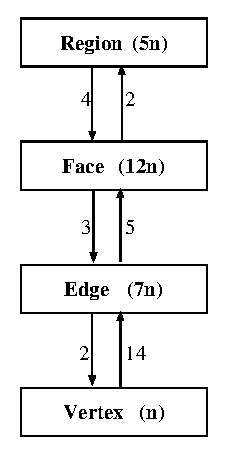
\includegraphics[scale=0.9]{figures/repF1} \\
        Representation F1
      \end{center}
    \end{minipage}
    \begin{minipage}{1.75in}
      \begin{center}
        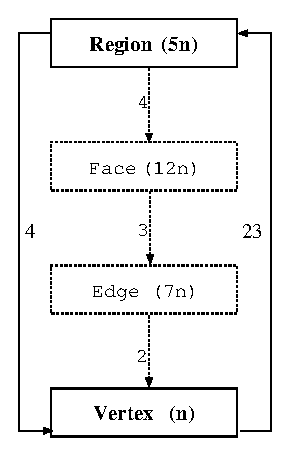
\includegraphics[scale=0.9]{figures/repR1} \\
        Representation R1
      \end{center}
    \end{minipage}
  \end{center}
  \label{fig:reptypes}
\end{figure}

\end{frame}

\begin{frame}
\frametitle{Mesh entity classification}

{\em Classification} - relationship of each mesh entity to the model
entity it represents the whole or a part of.

\begin{figure}
  \begin{center}
    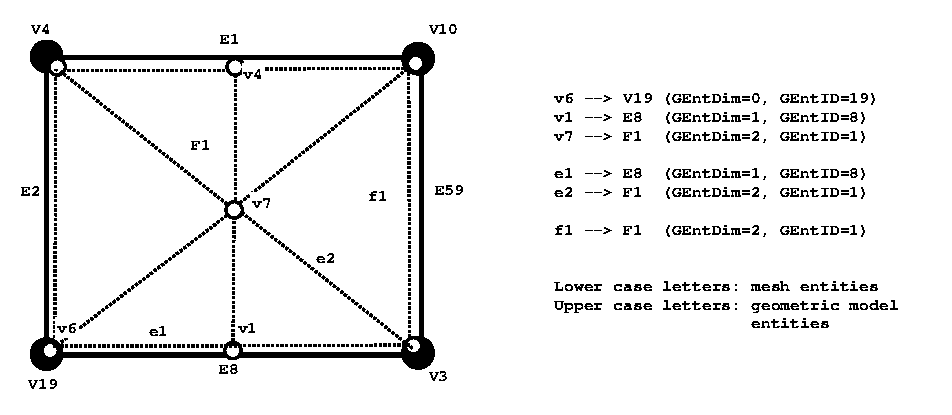
\includegraphics[width=\textwidth]{figures/classfn}
  \end{center}
  \caption{Example mesh and model showing the classification of mesh entities on geometric model entities}
\end{figure}

\end{frame}

\begin{frame}
\frametitle{Mesh entity classification - continued}

\begin{itemize}
\item Classification useful for simplifying algorithms in meshing and
  analysis applications.
  \begin{itemize}
  \item Specialization of mesh operations such as smoothing on
    boundary of domain
  \item Checking for topological conformity and guarding against
    dimensional reduction in mesh modification
  \item Assignment of material properties
  \item Application of boundary conditions
  \end{itemize}
\item Where possible, applications should supply classification data
\item If unavailable, classification of entities can be derived based
  on ``material IDs'' - but its not foolproof
\end{itemize}

\end{frame}

\begin{frame}
\frametitle{Parallel Mesh Management}

\begin{itemize}
\item Support for surface and volume meshes distributed across arbitrary number of processors
\item Currently allows one (or no) layer of overlapped or ghost entities around each partition
\item Ghost layers support all entities and connectivities
\item Mesh can be imported/created on processor 0 and distributed to other processors
\item Mesh can be partitioned using Metis or Zoltan
\item Meshes that are very thin in one direction can be partitioned in lateral direction only
\item Pre-partitioned mesh can be read on each processor and ``woven'' together to establish interprocessor connectivity
\item Support for updating vertex coordinates or attributes across processors
\item No support yet for parallel mesh modification
\end{itemize}

\end{frame}

\begin{frame}
\frametitle{Getting meshes in and out of MSTK}

Import:
\begin{itemize}
\item MSTK (Can convert to different representation in import)
\item Exodus II (serial)
\item Exodus II/Nemesis I (parallel)
\item GMV (General Mesh Viewer)
\end{itemize}

Export:
\begin{itemize}
\item MSTK (Can convert to different representation in export)
\item Exodus II(serial)
\item Exodus II/Nemesis I (parallel)
\item GMV
\item STL
\item FLAG X3D
\end{itemize}

Standalone tool 'meshconvert' can also be used for partitioning meshes
and converting between formats.
\end{frame}

\begin{frame}
\frametitle{MSTK based Applications and Software}

\begin{itemize}
  \item Subsurface flow and reactive transport (Amanzi)
  \item Arctic Terrestrial Simulator to study effects of warming on
  arctic permafrost (ATS)
  \item Unstructured polyhedral mesh optimization and untangling (optmesh)
  \item Adaptive Mesh Refinement in 2D
  \item Polyhedral Mesh Generation
  \item Interface Reconstruction
  \item Mimetic Finite Difference based solver for elliptic problems
\end{itemize}

\end{frame}

\begin{frame}
\frametitle{MSTK Computational Cost}

Amanzi software for subsurface flow and transport incorporates three
different mesh frameworks - MSTK (LANL), STKmesh (SNL) and MOAB
(ANL\/U.of.Wisc).

Computational cost of Amanzi's components with the three frameworks
for a subsurface flow problem is shown below:

\begin{figure}
\begin{center}
\includegraphics[scale=0.8]{figures/AmanziPerf-MSTK-STK-MOAB.pdf}
\end{center}
\end{figure}

Graph shows performance without (left 3 columns) and with (right 3
columns) caching of frequently used mesh data within Amanzi.

\end{frame}

\begin{frame}
\frametitle{MSTK Memory Usage}

The memory usage of MSTK (using the full F1 representation) compared
to STKmesh (SNL) and MOAB (ANL\/U.of.Wisc) for a simple subsurface flow
problem in Amanzi is shown below (statistics collected by Massif):

\begin{table}
  \begin{center}
  \begin{tabular}{|c|c|c|}
    \hline%
    MSTK & STK-Mesh & MOAB \\
    \hline
    165 MB  & 195 MB  &  240 MB \\
  \hline
  \end{tabular}
  \end{center}
  \label{tab:memtable}
\end{table}

MSTK's memory usage for a million elements on a 64-bit machine (no
extra application data) is as shown:

\begin{table}
  \begin{center}
  \begin{tabular}{|c||c|c|}
    \hline%
     {} & F1 representation & R1 representation \\
    \hline%
    1 Million Tetrahedra  &  650 MB  &  210 MB \\
    1 Million Hexahedra  & 1400 MB  &  430 MB \\
    \hline
  \end{tabular}
  \end{center}
  \label{tab:memtable}
\end{table}

\end{frame}

\begin{frame}
\frametitle{Parallel Scaling}

\end{frame}


\begin{frame}[fragile]
\frametitle{Example program - Initialize mesh}

\begin{verbatim}
#include "MSTK.h"

int main(int argc, char *argv[]) {
 int i, idx, idx2, ok, edir;
 double xyz[3];
 char meshname[256] = "testmesh.mstk";
 Mesh_ptr mesh;
 MVertex_ptr v;
 MEdge_ptr e;
 MFace_ptr f;
  
 MSTK_Init(); /* Initialize MSTK */

 mesh = MESH_New(UNKNOWN_REP);          /* Create a mesh object */
 if (!(ok = MESH_InitFromFile(mesh,meshname)) { /* Load the mesh */
   fprintf(stderr,"Cannot load input file %s\n\n\n",meshname);
   exit(-1);
 }

\end{verbatim}
\end{frame}

\begin{frame}[fragile]
\frametitle{Example (contd.) - Print vertex information}

\begin{verbatim}
 int nv = MESH_Num_Vertices(mesh);
 for (i = 0; i < nv; i++) \{
  v = MESH_Vertex(mesh,i);

  /* Basic info */
  printf("\nVertex: 0x%-x   ID: %-d   ", v, MV_ID(v));
  
  /* Classification w.r.t. geometric model */
    
  int gdim = MV_GEntDim(v);
  int gid = MV_GEntID(v);
  printf("GEntID: %-d   GEntDim: %-d\n", gid, gdim);

  MV_Coords(v,xyz);   /* Coordinates */
  printf("Coords: %16.8lf %16.8lf %16.8lf\n",xyz[0],xyz[1],xyz[2]);
 \}
\end{verbatim}
\end{frame}

\begin{frame}[fragile]
\frametitle{Example (contd.) - Print face information}

\begin{verbatim}
 idx = 0;
 while ((f = MESH_Next_Face(mesh,&idx))) {

  printf("\nFace: 0x%-x   ID: %-d   ", f, MF_ID(f)); 
  
  printf("Vertex IDs:\n");
  List_ptr fvertices = MF_Vertices(f,1,0);

  idx2 = 0;
  while ((v = List_Next_Entry(fvertices,&idx2)))
    printf("%-d\n",MV_ID(v));
  printf("\n");

  List_Delete(fvertices);
 }

 MESH_Delete(mesh);
 return 1;
}
\end{verbatim}
\end{frame}

\begin{frame}
\frametitle{Acknowledgements}

This work was performed under the auspices of the National Nuclear
Security Administration of the US Department of Energy at Los Alamos
National Laboratory under contract No. DE-AC52-06NA25396 as part of
projects funded by the DOE Office of Science SciDAC program, the DOE
Advanced Simulation Capability (ASC) program, the DOE Advanced
Simulation Capability for Environmental Management (ASCEM) program and
Los Alamos National Laboratory LDRD program.

\end{frame}


\end{document}
